\section{Metodología}\label{sec-metodología}

Como se ha apuntado con anterioridad, este estudio se aproxima, desde
una perspectiva bibliográfica, al impacto que tiene la tecnología sobre
el aprendizaje del alumnado de Educación Superior en el contexto
iberoamericano.

La estrategia de búsqueda y selección de los artículos se ha centrado en
la base de datos Dialnet por su prestigio, así como su alcance
geográfico. En cuanto a los términos de búsqueda, se han planteado
\enquote{tecnología}, \enquote{aprendizaje}, \enquote{educación superior} y
\enquote{competencias}, tanto en español, como en portugués e inglés. La
búsqueda ha arrojado un total de 924 resultados, que han sido filtrados
en base a los criterios que se refieren en la \Cref{tab-01}:

\begin{table}[h!]
\caption{Criterios de selección de documentos.}
\label{tab-01}
\centering
\begin{tabular}{l|lp{5cm}}
Tipología & Artículos científicos& Se descartan otro tipo de publicaciones \\
Disponibilidad & Acceso abierto y texto completo & Se descarta el pago por el acceso\\
Tipo de estudio & Investigación empírica & Se descartan estudios teóricos o metaestudios\\
Participantes & Alumnado de E. superior & Se descartan otros participantes\\
Fecha de publicación & 2021-2023 & Se descartan estudios publicados en años anteriores y posteriores\\
Contexto geográfico & Iberoamérica & Se descartan publicaciones de otros contextos\\
Idioma & Español, portugués o inglés & Se descartan otros idiomas\\
\end{tabular}
\source{Elaboración propia.}
\end{table}

Se realizo, a continuación, una~búsqueda inversa, pero no se hallaron
propuestas ajustadas a los criterios definidos. En la \Cref{fig-01} se
detalla el proceso de búsqueda y selección seguido, basado en el método
PRISMA \cite{urrutia2010}:


\begin{figure}[h!]
\caption{Proceso de selección de documentos.}
\label{fig-01}
\centering
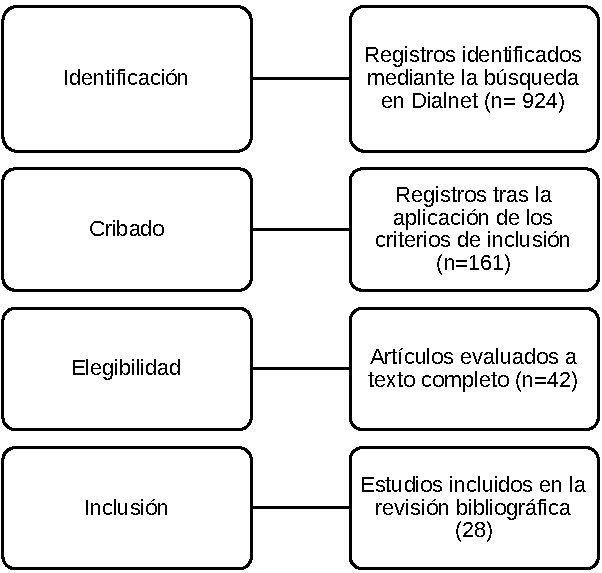
\includegraphics[width=.5\textwidth]{image1.pdf}
\source{Elaboración propia.}
\end{figure}
       

Estos 28 documentos son objeto de análisis de contenido, explorando de
manera específica las variables que se detallan en la \Cref{tab-02}:

\begin{table}[h!]
\centering
\caption{Variables de análisis.}
\label{tab-02}
\begin{tabular}{p{3cm}lp{7cm}}
\toprule
\multirow{4}{=}{Variables identificativas} & Fecha& Año de publicación \\ 
  & País & Contexto geográfico de la investigación\\
  & Autoría & Relación de autores y coautores\\
  & Idioma & Lengua en que se publica el artículo\\
\midrule
\multirow{4}{=}{Variables de contenido} & Muestra & Participantes del estudio\\
  & Objetivos & Fines que persigue el estudio\\
  & Tecnología & Herramienta digital utilizada\\
  & Resultados & Principales hallazgos del estudio\\
\bottomrule
\end{tabular}
\source{Elaboración propia.}
\end{table}


